\chapter{Exercise Games}
In this chapter we will present what exercise games are and how it can be used for exercising. To understand the concept of exergames and where it originates from, we will start with a brief presentation of what video games and serious games are. We will also present the technology that will be used for the game we are developing a concept for, namely Microsoft Kinect. 

\section{Video Games}

Video games are a genre within digital games that has become extremely popular all over the world. There exist several different gaming consoles, and for each console there has been developed an endless amount of various games that meets almost every need and interest. Video games can be described as \emph{"electronic, interactive games known for their vibrant colors, sound effects, and complex graphics"} \cite{videogamedef}. Hand held controllers or devices that capture movement are used to interact with the video game. The variety of video games makes it usable for many different purposes, like learning, education, physical activity, or just for the sake of amusement \cite{project}. 

One might associate video games with children and teenagers, and many hours of game play. Generally, this is a right assumption to make. In USA, video games are played for several hours every day \cite{foxnews}, and one third of all gamers are under the age of 18 \cite{videogames2012}. Gaming are usually associated with being anti-social, because of all the time spent looked up alone in a room, playing. However, the gaming lifestyle have changed. Video games has emerged from sedentary, lonely gaming, to gaming involving social interaction and movement, and it has taken a great part in people's everyday life. In Norway, 6 percent of the population in the age range 45 - 79 use computer or video games every day \cite{mediebarometer2012}. This might indicate that not only children and teenagers uses video games, but also the elderly population have started to use this type of technology. Statistics from USA in 2011 provided numbers that might support this assumption, as they showed that as much as 29 percent of all gamers where over the age of 50 \cite{videogames2011}. Elderly contributes to a great share of the world's population, and if the entertainment industry could see this group as potential customers, it would open up a new and inexperienced market for video games \cite{ijsselsteijn2007digital}. 

\section{Serious Games}
\label{sec:sergames}
The widespread and assorted use of video games have made a great potential for the entertainment industry regarding development of new games, and also in terms of developing games for additional purposes beside pure entertainment. A new way to use video games is to include it in training, education and learning. This is called serious games. Serious games can be described as \emph{"a mental contest, played with a computer in accordance with specific rules, that uses entertainment to further government or corporate training, education, health, public policy, and strategic communication objectives"} \cite{zyda2005visual}. The idea is to use the fun, motivating and captivating features that video games possess and combine it with pedagogy. If a video game can be defined as a serious game depends on how the game is used, the purpose of the game and the users gaming experience. 

The first serious attempt in developing video games with the main focus on learning did not become very successful \cite{understandingvg}. The failure that time was that the focus in these  video games were on pure learning, which resulted in boring games that did not create motivation and curiosity \cite{understandingvg} \cite{susi2007serious}. Michael Zyda states that, in serious games, pedagogy has to be subordinate to the story and entertainment component of the game. It is highly important that fun and amusement is the main focus in the game \cite{zyda2005visual}. For a video game to function as a pedagogical tool it has to focus on motivation, effectiveness, debriefing, and intuitiveness. These games have to provide motivating factors that engage people to play the game, and they have to be effective in the matter of learning outcome. Debriefing has the intention of creating a state of mind where thoughts and feelings are processed after playing the game, and when it comes to intuitiveness, people have to be able to play and understand the video games without the need for guidance \cite{understandingvg}. 

There exist several genres of serious games, where edutainment and game-based learning, advertaintment, games for politics, simulation games, and games for health are some of them. The genre of edutainment and game-based learning combines fun and entertainment with education and learning. Advertainment is about using video games as a media for marketing, and games for politics influences players through hidden, underlying political messages in the game. Simulation games are about bringing various activities into life with the use of video games, and gaming for health is about using video games to engage activity, to become physically stronger, and to improve quality of life. Gaming for health includes a topic called exercise games, which has training as a main focus \cite{understandingvg} \cite{alfingewang}.

An important feature with serious games is that they provide the opportunity to experience real-life situations and adventures one may otherwise not be able to enjoy. This might be due to expenses, time, distance, risk, or physical capabilities. With serious games it is possible to play golf, be the star of a boxing match, paddle down turbulent rivers, and explore nature and creatures one have never seen before. In a more serious matter, video games can be used to simulate brain surgery or a battle in a war zone. This can teach students how to perform medical procedures or it could prepare soldiers for war. Serious games can also be used for students to learn their curriculum through quiz games, and people can be motivated to work out with exercise games. Serious games can be used for several purposes and situations, and it can help people develop a wide range of different skills. 

Research on the use of serious games show positive development of skills and knowledge, in addition to positive effect on health, which have resulted in motivation for further research and development. In addition, the new technology involving physical interfaces and improvement on graphics and animations initiates to new types of games. The market for serious games are inexperienced and unexplored, so there are a great potential for further research \cite{alfingewang}. Market sales the last couple of years also shows promise for serious video games in the future. In 2008, the market for serious games sold for around 1,5 billion USD around the globe \cite{alfingewang}, and in 2010 it reached about 2 billion USD (1,5 billion EUR). The market is expecting a annual growth rate of 47 percent, up to impressive 13,5 billion USD (10 billion EUR) in 2015 \cite{idate}. 

We will look closer into one of the genres within serious games, exercise games.  

\section{Exergames}
\label{sec:exergames}
Exergames are a type of serious video games that combine traditional game play with physical activity. The combination of movement and amusement is used to stimulate exercise and engage people to be more physically active in a fun and motivating way. A lot of research have been done within this topic, and results show that exergames can have a positive effect on users health. In addition to being a new, and more amusing way to work out, exergames provide an opportunity for social interaction. A great amount of today's existing computer and video games possess this feature, and as much as 62 percent of all gamers say they play with others either in-person or online. One of the two top-selling video games in 2011 was Just Dance 3, which is an exergame that has the possibility to play with others \cite{statistics2012}. This shows that the social aspect of gaming is important. The social aspect these games provide may also be especially important for people who experience loneliness in their everyday life \cite{exergamesforelderly}.

Exergames use technology like remote hand held controllers and motion sensors to capture body movements. Users are therefore required to get up and move their body to be able to play the game. There exist several consoles that support this technology, where Nintendo Wii, Playstation Move, Dance Dance Revolution and Xbox Kinect are some of them. The existing consoles use different type of devices to capture body movement, like hand held controllers, different boards and pads with embedded sensors, and video cameras with motion sensors. In this assignment we will focus on the Kinect sensor technology. This is because we in our previous project evaluated Kinect to be an appropriate choice as it provides the possibility to play without holding on to any devices, and because the sensor has proved to measure different body movements accurately so that the parameters are applicable for use in clinical practice. The reader will be referred to our project assignment \cite{project} and Section 4.2 to read what this is based on. We will now provide a brief description of the chosen technology.

\section{Microsoft Kinect for Xbox 360 and Windows}
Microsoft Kinect is a motion sensor that captures movement without the use of any controllers. This gives players the opportunity to play and interact with the game only by gestures and body movement. Xbox presents the Kinect experience this way: \emph{"Kinect for Xbox 360 brings games and entertainment to life in extraordinary new ways without using a controller"} \cite{kinectxboxdef}. The word Kinect is a fusion of two words, \emph{kinetic}, which means movement, and \emph{connect}, which relates to the social aspect \cite{howstuffworksKinect}. The Kinect sensor was released by Microsoft in November 2010 as an input device to the Xbox 360 console, and it did not take long before the Microsoft Kinect got extremely popular. Only ten days after the release in 2010 it had been sold 1 million Kinect motion sensors, and in January 2012, sales numbers had climbed up to over 18 million sold units \cite{kinectsales}. These sales numbers put Kinect into history, as no other consumer electronic device has experienced such great sales numbers in such a short amount of time. The Kinect sensor has the possibility to be used without the Xbox 360 console, as it also is compatible with Windows computers. A more detailed information about developing for Kinect, and a presentation of the technology provided by the Kinect Sensor, will for the interested reader be presented in Appendix A.

\begin{figure} 
\centering
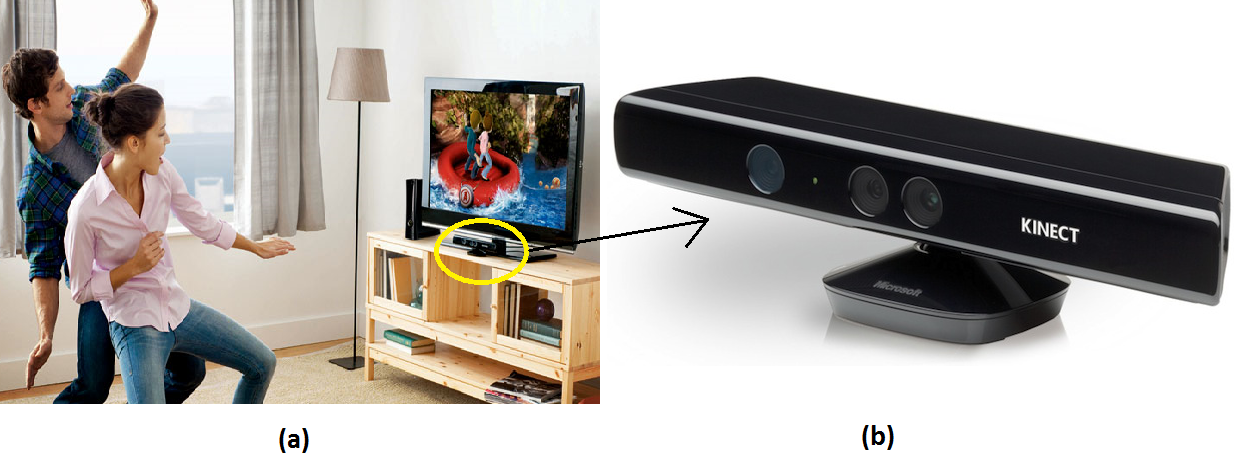
\includegraphics[scale=0.36]{sensorandtv}
\caption[The Kinect sensor]{The Kinect sensor (a) together with the rest of the needed equipments, and (b) alone}
\label{kinectsensor}
\end{figure} 
 
Kinect has not just experienced success as an entertainment device within the living room, researches have also started to see the possibility to use the Kinect for other non-gaming purposes, like within healthcare, education and industry. The key reasons for the broad use of Kinect are its accessibility and low price, in addition to the ground breaking technology it provides. The release of the Kinect for Windows \ac{sdk} is also a reason for the wealth of non-gaming applications, as it makes the the Kinect platform available for everyone to develop on \cite{microsoftnews}. 

